%%%%%%%%%%%%%%%%%%%%%%%%%%%%%%%%%%%%%%%%%
% Beamer Presentation
% LaTeX Template
%%%%%%%%%%%%%%%%%%%%%%%%%%%%%%%%%%%%%%%%%

%----------------------------------------------------------------------------------------
%	PACKAGES AND THEMES
%----------------------------------------------------------------------------------------

\documentclass[aspectratio=169]{beamer}

\mode<presentation> {

% The Beamer class comes with a number of default slide themes
% which change the colors and layouts of slides. Below this is a list
% of all the themes, uncomment each in turn to see what they look like.

%\usetheme{default}
%\usetheme{AnnArbor}
%\usetheme{Antibes}
%\usetheme{Bergen}
%\usetheme{Berkeley}
%\usetheme{Berlin}
%\usetheme{Boadilla}
%\usetheme{CambridgeUS}
%\usetheme{Copenhagen}
%\usetheme{Darmstadt}
%\usetheme{Dresden}
%\usetheme{Frankfurt}
%\usetheme{Goettingen}
%\usetheme{Hannover}
%\usetheme{Ilmenau}
%\usetheme{JuanLesPins}
%\usetheme{Luebeck}
\usetheme{Madrid}
%\usetheme{Malmoe}
%\usetheme{Marburg}
%\usetheme{Montpellier}
%\usetheme{PaloAlto}
%\usetheme{Pittsburgh}
%\usetheme{Rochester}
%\usetheme{Singapore}
%\usetheme{Szeged}
%\usetheme{Warsaw}

% As well as themes, the Beamer class has a number of color themes
% for any slide theme. Uncomment each of these in turn to see how it
% changes the colors of your current slide theme.

%\usecolortheme{albatross}
%\usecolortheme{beaver}
%\usecolortheme{beetle}
%\usecolortheme{crane}
%\usecolortheme{dolphin}
%\usecolortheme{dove}
%\usecolortheme{fly}
%\usecolortheme{lily}
%\usecolortheme{orchid}
%\usecolortheme{rose}
%\usecolortheme{seagull}
%\usecolortheme{seahorse}
%\usecolortheme{whale}
%\usecolortheme{wolverine}

%\setbeamertemplate{footline} % To remove the footer line in all slides uncomment this line
\setbeamertemplate{footline}[page number] % To replace the footer line in all slides with a simple slide count uncomment this line

\setbeamertemplate{navigation symbols}{} % To remove the navigation symbols from the bottom of all slides uncomment this line
}

\usepackage{graphicx,tabularx,multirow,tikz} % Allows including images
\usepackage{booktabs} % Allows the use of \toprule, \midrule and \bottomrule in tables
%\usepackage {tikz}
\usepackage{tkz-graph,xcolor}
\GraphInit[vstyle = Shade]
%\tikzset{
%  LabelStyle/.style = { rectangle, rounded corners, draw,
%                        minimum width = 2em, fill = yellow!50,
%                        text = red, font = \bfseries },
%  VertexStyle/.append style = { inner sep=5pt,
%                                font = \normalsize\bfseries},
%  EdgeStyle/.append style = {->, bend left} }
\usetikzlibrary {positioning}
\usetikzlibrary{snakes}
\usetikzlibrary{calc}
\usetikzlibrary{arrows}
\usetikzlibrary{decorations.markings}
\usetikzlibrary{shapes.misc}
\usetikzlibrary{matrix,shapes,arrows,fit,tikzmark}
\usepackage{lmodern}
\usepackage[beamer,customcolors]{hf-tikz}

\tikzset{hl/.style={
    set fill color=red!80!black!40,
    set border color=red!80!black,
  },
}


%\usepackage {xcolor}
\definecolor {processblue}{cmyk}{0.96,0,0,0}


%----------------------------------------------------------------------------------------
%	TITLE PAGE
%----------------------------------------------------------------------------------------

\title[Short title]{Collective Action, Communication and the Coordination Challenge:
An Analysis of Smallholder Livestock Cooperatives in Nepal \\
{\small Dissertation Proposal}} % The short title appears at the bottom of every slide, the full title is only on the title page

\author{Scott M. Miller} % Your name
\institute[Food and Resource Economics Department, University of Florida] % Your institution as it will appear on the bottom of every slide, may be shorthand to save space
{
Food and Resource Economics Department \\ University of Florida\\ % Your institution for the title page
\medskip
}
%\date{} % Date, can be changed to a custom date
\newenvironment{wideitemize}{\itemize\addtolength{\itemsep}{10pt}}{\enditemize}

\begin{document}

\begin{frame}
\titlepage % Print the title page as the first slide
\end{frame}

%\begin{frame}
%\frametitle{Overview} % Table of contents slide, comment this block out to remove it
%\tableofcontents % Throughout your presentation, if you choose to use \section{} and \subsection{} commands, these will automatically be printed on this slide as an overview of your presentation
%\end{frame}

%----------------------------------------------------------------------------------------
%	PRESENTATION SLIDES
%----------------------------------------------------------------------------------------


%------------------------------------------------
\section{Introduction}

\begin{frame}{Introduction}
    \begin{wideitemize}
        \item Two-thirds of the world’s poorest households live in rural areas and depend on agriculture for their livelihoods (Fuglie et al., 2019). 
        \item Rural markets in developing countries are often rife with constraints that limit the ability of smallholders to sell in formal markets (Ashby et al., 2009; Kristjanson et al., 2014). \vspace{.25cm}
            \begin{itemize}
                \item Poor infrastructure, weak communication channels and long distances between market actors. \vspace{.25cm}
                \item High transaction costs, weak bargaining power and information asymmetry (Aker, 2010; Barrett, 2008; Key et al., 2000; Staal et al., 1997).
            \end{itemize}
    \end{wideitemize}
\end{frame}

\begin{frame}{Introduction}
    \begin{wideitemize}
        \item Agricultural cooperatives often arise in an effort to increase bargaining power, decrease transaction costs, and help achieve scale economies in marketing (Markelova et al., 2009; Rondot and Collion, 2001; Staal et al., 1997; World Bank, 2003).
        \item Through collective action, cooperatives give smallholders the potential to: \vspace{.25cm}
            \begin{enumerate}
                \item Access markets that may otherwise be inaccessible. \vspace{.25cm}
                \item Pool resources to overcome financial constraints. \vspace{.25cm}
                \item Increase communication flows to combat information asymmetries. \vspace{.25cm}
                \item Collectively negotiate with buyers to receive better prices (Poole and De Frece, 2010).
            \end{enumerate}
    \end{wideitemize}
\end{frame}

\begin{frame}{Introduction}
    \begin{wideitemize}
        \item Cooperatives don't eliminate market constraints. \vspace{.25cm}
            \begin{wideitemize}
                \item Shift constraints from individual market actors to the cooperatives (Coase, 1937). 
            \end{wideitemize}
        \item Success of cooperatives is determined by their ability to coordinate sales among a large group of individual market actors (``Coordination Challenge''). 
        \item Evidence shows a large disparity: \vspace{.25cm}
            \begin{wideitemize}
                \item Generate large and inclusive benefits for their members (Narrod et al., 2009; Tadesse and Bahiigwa, 2015; Wollni and Zeller, 2007). 
                \item High presence of side-selling, heterogeneous benefits, or dissolving participation among their members (Aflagah et al., 2019; Bernard and Spielman, 2009; Casaburi and Macchiavello, 2015).
            \end{wideitemize}
    \end{wideitemize}
\end{frame}


\begin{frame}{Introduction}

\textbf{Research Question:} \vspace{.5cm}
    \begin{wideitemize}
        \item Which factors influence the success and failure of agricultural cooperatives and how can researchers, policymakers and NGOs promote thriving producer organizations? \vspace{.25cm}
            \begin{enumerate}
                \item Decompose the cooperative performance gap between the most and least inclusive cooperatives. \vspace{.25cm}
                \item Analyze the role that comparative advantage plays in cooperative participation decisions. \vspace{.25cm}
                \item Assess the impacts of a smartphone application that is designed to improve cooperative performance.
            \end{enumerate}
    \end{wideitemize}
\end{frame}

% -------------------------------------------------
\section{Background \& Data}

\begin{frame}{Background \& Data}
    \begin{wideitemize}
        \item Female smallholder goat producers in rural Nepal. All are members of cooperatives. 
        \item In Nepal, 68\% of the population depends on agriculture for their livelihoods (International Labor Organization, 2016). 
        \item Nearly every rural household owns a least a few goats for production and/or consumption (Upreti, 2009). 
        \item A recent rise in demand for goat meat \vspace{.25cm}
        \begin{wideitemize}
            \item Domestic production has been unable to keep up with rising demand, leading to higher imports from India and Tibet (Heifer International Nepal, 2012).
        \end{wideitemize}
    \end{wideitemize}
\end{frame}

\begin{frame}{Background \& Data}
\textbf{Data:} \vspace{.5cm}
    \begin{wideitemize}
        \item 109 female smallholder livestock cooperatives. 
        \item Two separate surveys: \vspace{.25cm}
            \begin{wideitemize}
                \item Household survey - 2,856 households, all members of the 109 cooperatives.
                \item Cooperative survey - 3 leaders from each cooperative (board member, general manager, chairwoman). 
            \end{wideitemize}
        \item Round 1 - January 2018 
        \item Round 2 - February 2020
    \end{wideitemize}
\end{frame}

\begin{frame}{Background \& Data}
    \begin{center}
        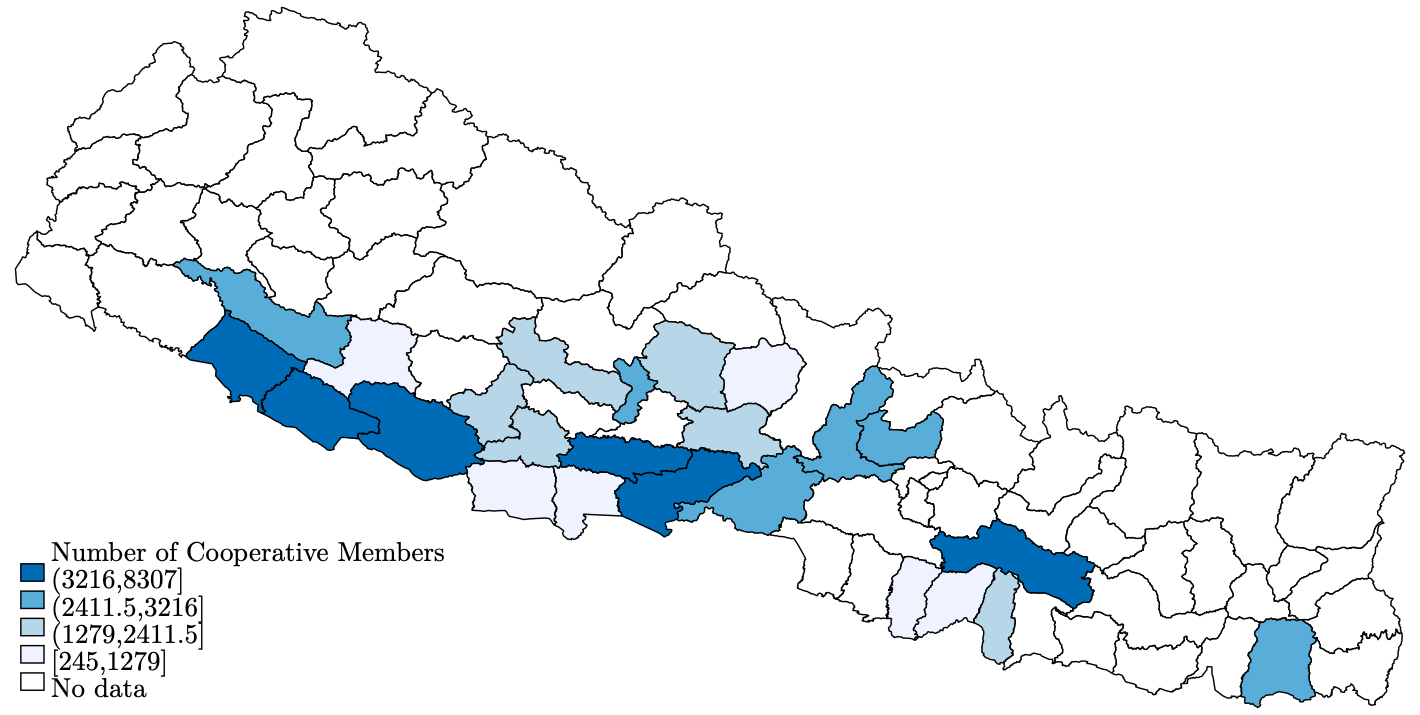
\includegraphics[width=.9\textwidth]{StudyMap.png}
    \end{center}
\end{frame}


% -------------------------------------------------
\section{Essay 1: ``Investigating the Inclusive-Performance Tradeoff in Agricultural Cooperatives.''}
\begin{frame}{Essay 1}
\centering
\Large{``Investigating the Inclusive-Performance Tradeoff in Agricultural Cooperatives.''}
\end{frame}


\begin{frame}{Essay 1: Investigating the Inclusive-Performance Tradeoff in \\ \hspace{1.7cm} Agricultural Cooperatives}

    \begin{wideitemize}
        \item The relationship between inclusive membership and market performance has been highlighted as an unresolved conflict in the cooperative literature (World Bank, 2008). 
        \item Bernard and Spielman (2009) suggest that cooperatives can achieve only two of the following three conditions: \vspace{.25cm}
            \begin{enumerate}
                \item Inclusive membership \vspace{.25cm}
                \item Participatory decision-making \vspace{.25cm}
                \item Market performance
            \end{enumerate}
        \item Previous literature has failed to account for selection bias, possibly obscuring the relationship of interest. 
    \end{wideitemize}
\end{frame}

\begin{frame}{Essay 1: Investigating the Inclusive-Performance Tradeoff in \\ \hspace{1.7cm} Agricultural Cooperatives}
    \begin{wideitemize}
        \item I propose to use the Oaxaca (1973)-Blinder (1973) decomposition to further examine this relationship. 
        \item Separate the performance gap between the most and least inclusive cooperatives in my sample into: \vspace{.25cm}
            \begin{itemize}
                \item the portion that is explained by differences in observable characteristics \vspace{.25cm}
                \item the portion that is explained by the returns to those characteristics
            \end{itemize}
    \end{wideitemize}
\end{frame}

\begin{frame}{Essay 1: Investigating the Inclusive-Performance Tradeoff in \\ \hspace{1.7cm} Agricultural Cooperatives}
    \begin{wideitemize}
        \item Decomposition methods closely follow the program evaluation literature (Fortin et al., 2011). 
        \item `Explained' portion of the gap is selection bias (differences in characteristics between two groups).
        \item ‘Unexplained’ portion of the gap is analogous to a treatment effect (Fortin et al., 2011). \vspace{.25cm}
            \begin{wideitemize}
                \item Not causal estimates
            \end{wideitemize}
    \end{wideitemize}
\end{frame}

\begin{frame}{Essay 1: Investigating the Inclusiveness-Performance \\ \hspace{1.7cm} Tradeoff in Agricultural Cooperatives}
    \begin{wideitemize}
        \item Suppose that the relationship between the outcome for producer $i$, $Y_i$, and a vector of the determinants of performance, $\mathbf{X}_i$, can be written as: \vspace{.25cm}
            \begin{equation} \label{eq:E1_1}
                Y_i = \beta \mathbf{X}_i + \varepsilon_i 
            \end{equation} 
        \item Most and least inclusive cooperatives likely have different $\beta$'s (i.e. ability to translate characteristics into performance). 
        \item Using the group-specific parameters, the difference between average outcomes for the most and least inclusive cooperatives is written as: \vspace{.25cm}
            \begin{equation} \label{eq:E1_2}
                \overline{Y}_{\ell} - \overline{Y}_{m} =  \beta_{\ell}\overline{\mathbf{X}}_{\ell} - \beta_{m}\overline{\mathbf{X}}_{m}
            \end{equation}  
            \begin{itemize}
                \item $m$: most inclusive cooperatives
                \item $\ell$: least inclusive cooperatives 
            \end{itemize}
    \end{wideitemize}
\end{frame}

\begin{frame}{Essay 1: Investigating the Inclusive-Performance Tradeoff in \\ \hspace{1.7cm} Agricultural Cooperatives}
    \begin{wideitemize}
        \item Rearranging this equation by adding and subtracting $\beta_{m}\overline{X}_{\ell}$ on both sides gives: \vspace{.25cm}
            \begin{subequations}
                \begin{align}
                \overline{Y}&_{\ell} - \overline{Y}_{m} \label{eq:E1_3a} \\
                &= \beta_{m}[\overline{\mathbf{X}}_{\ell} - \overline{\mathbf{X}}_{m}] \label{eq:E1_3b} \\
                &+ \overline{\mathbf{X}}_{\ell}[\beta_{\ell} - \beta_{m}] \label{eq:E1_3c}
                \end{align}
            \end{subequations}  
        \item (\ref{eq:E1_3b}) is the explained component \vspace{.25cm}
            \begin{wideitemize}
                \item Difference between the average outcomes that producers in the most inclusive cooperatives actually receive, and what they could receive if their characteristics matched those of producers in the least inclusive cooperatives.
            \end{wideitemize}
    \end{wideitemize}    
\end{frame}

\begin{frame}{Essay 1: Investigating the Inclusive-Performance Tradeoff in \\ \hspace{1.7cm} Agricultural Cooperatives}
        \addtocounter{equation}{-1}
        \begin{subequations}
            \begin{align}
                \overline{Y}&_{\ell} - \overline{Y}_{m} \label{eq:E1_3a} \\
                &= \beta_{m}[\overline{\mathbf{X}}_{\ell} - \overline{\mathbf{X}}_{m}] \label{eq:E1_3b} \\
                &+ \overline{\mathbf{X}}_{\ell}[\beta_{\ell} - \beta_{m}] \label{eq:E1_3c}
            \end{align}
        \end{subequations}  
    \begin{wideitemize}
        \item (\ref{eq:E1_3c}) is the unexplained component \vspace{.25cm}
             \begin{wideitemize}
                \item Difference in what producers in the least inclusive cooperatives actually receive and what they would receive if they had equivalent returns to their characteristics as those in the most inclusive cooperatives.
            \end{wideitemize}
    \end{wideitemize}    
\end{frame}

\begin{frame}{Essay 1: Investigating the Inclusive-Performance Tradeoff in \\ \hspace{1.7cm} Agricultural Cooperatives}
    \begin{wideitemize}
        \item Also important to disentangle the role that institutional and individual characteristics play in explaining this performance gap. 
        \item I expand the above framework to include two separate vectors of attributes: one institutional and one individual. 
        \item I propose to estimate two separate specifications: \vspace{.25cm}
            \begin{enumerate}
                \item Pooled cross section
                    \begin{wideitemize}
                        \item Takes into account the full dataset \vspace{.25cm}
                    \end{wideitemize}
                \item First-difference panel
                    \begin{wideitemize}
                        \item Emphasize market performance in growth terms
                    \end{wideitemize}
            \end{enumerate}
    \end{wideitemize}    
\end{frame}

\begin{frame}{Essay 1: Investigating the Inclusive-Performance Tradeoff in \\ \hspace{1.7cm} Agricultural Cooperatives}
\textbf{Pooled Cross Section} \vspace{1cm}
        \begin{equation} \label{eq:E1_4}
            Y_{ij} = \mathbf{X}_i^{\prime}\beta + \mathbf{Z}_j^{\prime}\gamma + \varepsilon_{ij}
        \end{equation}  
    \begin{wideitemize}    
        \item $Y_{ij}$ - outcome of interest for individual $i$ who is a member of cooperative $j$
        \item $\mathbf{X}_i$ - vector of individual attributes
        \item $\mathbf{Z}_j$ is a vector of institutional attributes
    \end{wideitemize}    
\end{frame}

\begin{frame}
        \begin{table}[H]
        \caption{Decomposition Components (Cross-Section)}
        \label{table:E1_1}
        \centering
        \scalebox{1}{
        \begin{tabular}{lc}
        \noalign{\smallskip} \hline \noalign{\smallskip}
        Gap Portion & Equation \\
        \noalign{\smallskip} \hline \noalign{\smallskip}
        Full & $\overline{Y}_{\ell} - \overline{Y}_{m}$ \\ \\
        Individual (All) & $\beta_{m}[\overline{\mathbf{X}}_{\ell} - \overline{\mathbf{X}}_{m}] + \overline{\mathbf{X}}_{\ell}[\beta_{\ell} - \beta_{m}]$ \\
        Individual (Characteristics) & $\beta_{m}[\overline{\mathbf{X}}_{\ell} - \overline{\mathbf{X}}_{m}]$ \\
        Individual (Returns) & $\overline{\mathbf{X}}_{\ell}[\beta_{\ell} - \beta_{m}]$ \\ \\
        Institutional (All) & $\gamma_{m}[\overline{\mathbf{Z}}_{\ell} - \overline{\mathbf{Z}}_{m}] + \overline{\mathbf{Z}}_{\ell}[\gamma_{\ell} - \gamma_{m}]$ \\
        Institutional (Characteristics) & $\gamma_{m}[\overline{\mathbf{Z}}_{\ell} - \overline{\mathbf{Z}}_{m}]$ \\
        Institutional (Returns) & $\overline{\mathbf{Z}}_{\ell}[\gamma_{\ell} - \gamma_{m}]$ \\
        \hline
        \end{tabular}}
        \end{table} 
\end{frame}

\begin{frame}{Essay 1: Investigating the Inclusive-Performance Tradeoff in \\ \hspace{1.7cm} Agricultural Cooperatives}
\textbf{First-Difference Panel} \vspace{.5cm}
            \begin{equation} \label{eq:E1_7}
                \Delta Y_{ij} = \Delta \mathbf{X}_i^{\prime}\beta + \Delta \mathbf{Z}_j^{\prime}\gamma + \mathbf{h}_i^{\prime}\delta + \mathbf{c}_i^{\prime}\theta + \Delta \varepsilon_{ij}
            \end{equation}  
    \begin{wideitemize}    
        \item $\Delta Y_{ij}$ $(= Y_{ij,t=1} - Y_{ij,t=0})$ - outcome of interest for individual $i$ in cooperative $j$
        \item $\Delta \mathbf{X}_i$ - vector of time-varying individual attributes
        \item $\Delta \mathbf{Z}_j$ - vector of time-varying institutional attributes
        \item $\mathbf{h}_i$ - vector time-invariant individual attributes
        \item $\mathbf{c}_i$ - vector time-invariant intitutional attributes
    \end{wideitemize}    
\end{frame}

\begin{frame}
        \begin{table}[H]
        \caption{Decomposition Components (Panel)}
        \label{table:E1_2}
        \centering
        \scalebox{1}{
        %\hspace{1.43in}
        \begin{tabular}{lc}
        \noalign{\smallskip} \hline \noalign{\smallskip}
        Gap Portion & Equation \\
        \noalign{\smallskip} \hline \noalign{\smallskip}
        Full & $\overline{\Delta Y}_{\ell} - \overline{\Delta Y}_{m}$ \\ \\
        Individual (All) & $\beta_{m}[\overline{\Delta \mathbf{X}}_{\ell} - \overline{\Delta \mathbf{X}}_{m}] + \overline{\Delta \mathbf{X}}_{\ell}[\beta_{\ell} - \beta_{m}]$ \\
        & $+ \delta_{m}[\overline{\mathbf{h}}_{\ell} - \overline{\mathbf{h}}_{m}] + \overline{\mathbf{h}}_{\ell}[\delta_{\ell} - \delta_{m}]$ \\ \\
        Individual (Characteristics) & $\beta_{m}[\overline{\Delta \mathbf{X}}_{\ell} - \overline{\Delta \mathbf{X}}_{m}] + \delta_{m}[\overline{\mathbf{h}}_{\ell} - \overline{\mathbf{h}}_{m}]$ \\
        Individual (Returns) & $\overline{\Delta \mathbf{X}}_{\ell}[\beta_{\ell} - \beta_{m}] + \overline{\mathbf{h}}_{\ell}[\delta_{\ell} - \delta_{m}]$ \\ \\
        
        Institutional (All) & $\gamma_{m}[\overline{\Delta \mathbf{Z}}_{\ell} - \overline{\Delta \mathbf{Z}}_{m}] + \overline{\Delta \mathbf{Z}}_{\ell}[\gamma_{\ell} - \gamma_{m}]$ \\
        & + $\theta_{m}[\overline{\mathbf{c}}_{\ell} - \overline{\mathbf{c}}_{m}] + \overline{\mathbf{c}}_{\ell}[\theta_{\ell} - \theta_{m}]$ \\ \\
        Institutional (Characteristics) & $\gamma_{m}[\overline{\Delta \mathbf{Z}}_{\ell} - \overline{\Delta \mathbf{Z}}_{m}] + \theta_{m}[\overline{\mathbf{c}}_{\ell} - \overline{\mathbf{c}}_{m}]$ \\
        Institutional (Returns) & $\overline{\Delta \mathbf{Z}}_{\ell}[\gamma_{\ell} - \gamma_{m}] + \overline{\mathbf{c}}_{\ell}[\theta_{\ell} - \theta_{m}]$\\
        \hline
        \end{tabular}}
        \end{table}   
\end{frame}

% -------------------------------------------------
\section{Essay 2: ``Side-Selling and the Returns to Cooperative Participation: The Role of Comparative Advantage.''}
\begin{frame}{Essay 2}
\centering
\Large{``Side-Selling and the Returns to Cooperative Participation: The Role of Comparative Advantage.''}
\end{frame}


\begin{frame}{Essay 2: Side-Selling and the Returns to Cooperative Participation: The Role of Comparative Advantage}

    \begin{wideitemize}
        \item One of the most apparent examples of the shortcomings of agricultural cooperatives is the high presence of side-selling that often takes place. 
        \item Nearly 80\% of goat-selling households in my sample choose to sell their goats to a local trader instead of through the cooperative of which they are a member. \vspace{.25cm}
         \begin{wideitemize}
             \item Evidence suggesting that households who sell their goats through the cooperative receive a higher price and sell more goats on average than side-selling households
         \end{wideitemize}
    \end{wideitemize}
\end{frame}

\begin{frame}{Essay 2: Side-Selling and the Returns to Cooperative Participation: The Role of Comparative Advantage}
\begin{figure}[!h]
  \label{fig:app}
  \hspace{-1.2cm}
  \begin{minipage}{.45\textwidth}
    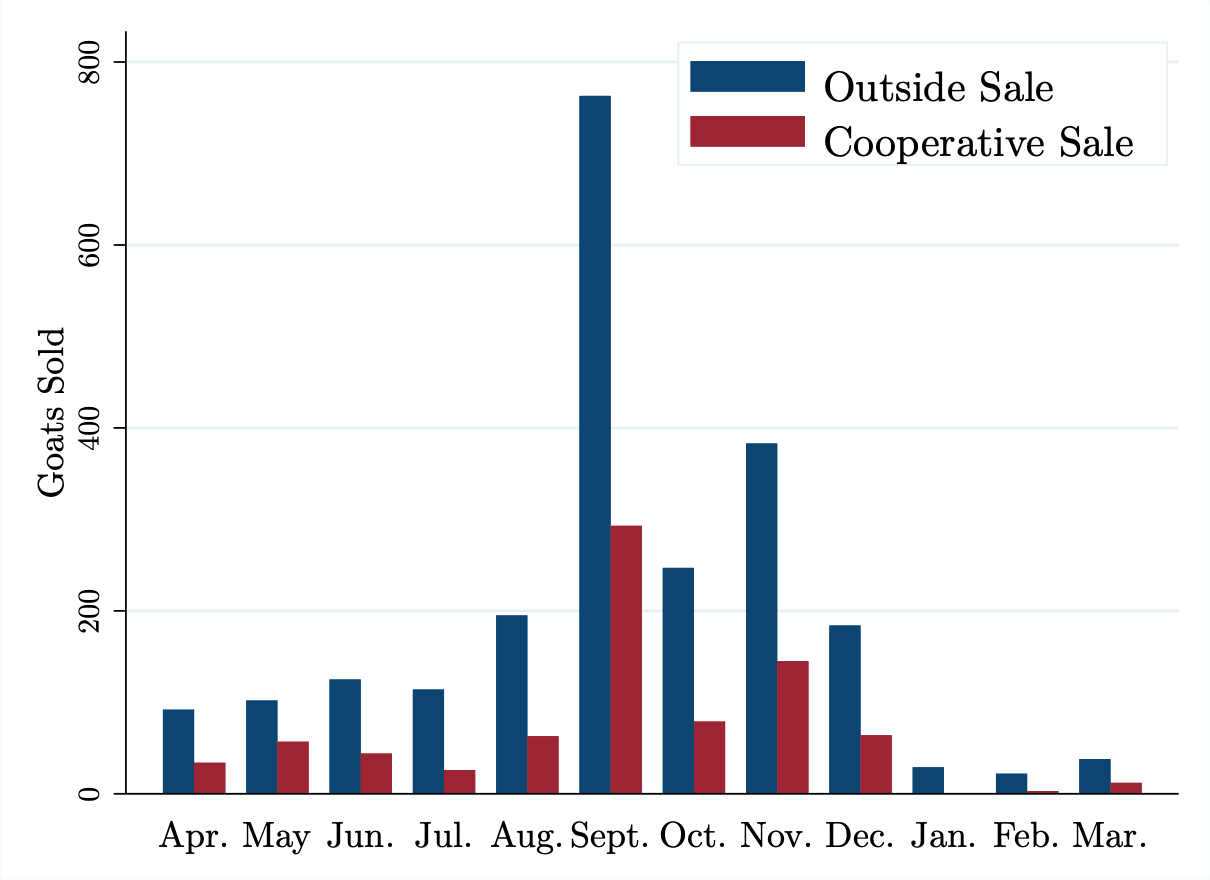
\includegraphics[width=7.6cm,trim=4 4 4 4,clip]{E2_SaleMonth.png}
  \end{minipage}
  \hspace{.5cm}
  \begin{minipage}{.45\textwidth}
  \vspace{.45cm}
    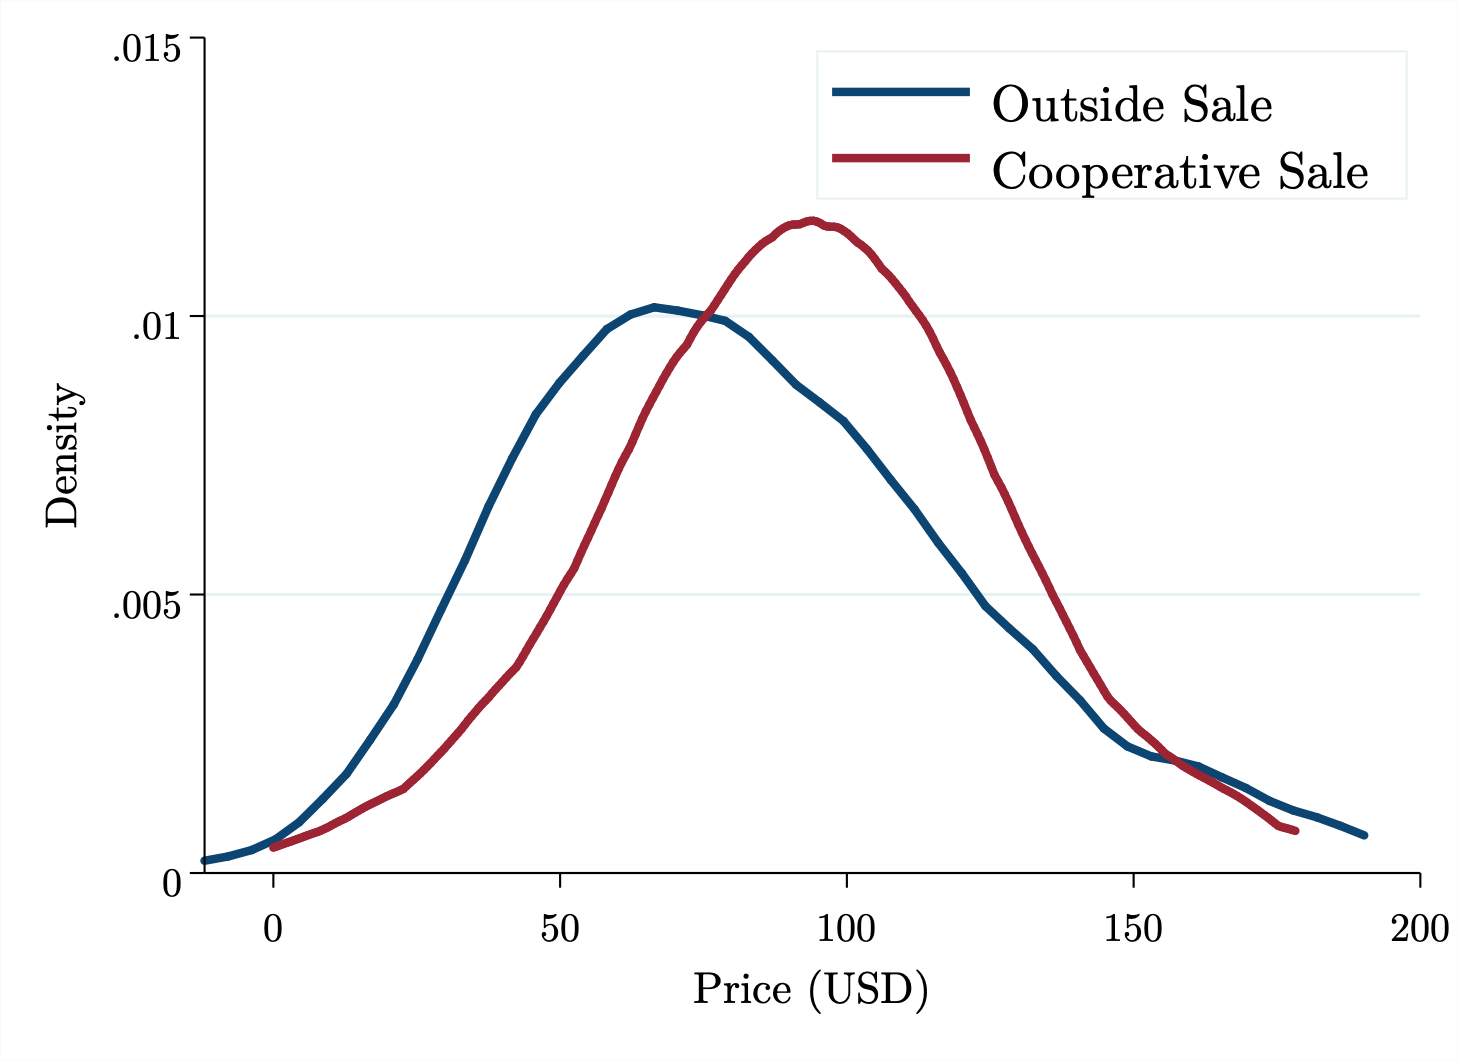
\includegraphics[width=7.6cm,trim=4 4 4 4,clip]{E2_PriceDensity_Annual.png}
  \end{minipage}
\end{figure}
\end{frame}

\begin{frame}{Essay 2: Side-Selling and the Returns to Cooperative Participation: The Role of Comparative Advantage}
    \begin{wideitemize}
        \item The goal of this paper is to empirically answer the following questions: \vspace{.25cm}
            \begin{enumerate}
                \item Are there significant net returns to selling through the cooperative? \vspace{.25cm}
                \item Are these returns heterogeneous? \vspace{.25cm}
                \item If so, does this heterogeneity explain why a small number of producers sell through the cooperative, and others side-sell? 
            \end{enumerate}
        \item I estimate a correlated random coefficient (CRC) model to analyze the distribution of net returns to cooperative sales and discuss the importance of comparative advantage in explaining the decision to do so.     
    \end{wideitemize}
\end{frame}

\begin{frame}{Essay 2: Side-Selling and the Returns to Cooperative Participation: The Role of Comparative Advantage}
    \begin{wideitemize}
        \item Suri, 2011. ``Selection and Comparative Advantage in Technology Adoption.''
 \vspace{.25cm}
            \begin{wideitemize}
                \item Explains why, despite high average returns to hybrid maize seed in Kenya, adoption of this technology was persistently low.
            \end{wideitemize}
        \item Michler et al., 2018. ``Money Matters: The Role of Yields and Profits in Agricultural Technology Adoption.''
 \vspace{.25cm}
            \begin{wideitemize}
                \item Conduct an extension test of Suri (2011) in the case of improved chickpea varieties in Ethiopia.
            \end{wideitemize}        
        \item Treat the decision to sell through the cooperative as a technology that producers are able to adopt.
    \end{wideitemize}
\end{frame}

\begin{frame}{Essay 2: Side-Selling and the Returns to Cooperative Participation: The Role of Comparative Advantage}
        \begin{wideitemize}
        \item Cobb-Douglas Production Function
        \begin{equation} \label{eq:E2_yield.C}
            Y^{C}_{it} = \beta^{C}_{t} + {X_{ijt}}^\prime \gamma^{C}_{i} + u^{C}_{it}
        \end{equation}   
        \begin{equation} \label{eq:E2_yield.O}    
            Y^{O}_{it} = \beta^{O}_{t} + {X_{ijt}}^\prime \gamma^{O}_{i} + u^{O}_{it}
        \end{equation}
        \item $Y^{C}_{it}$ and $Y^{O}_{it}$ are the quantity of goats sold through the cooperative (C) and outside of the cooperative (O)
        \item ${X_{ijt}}^\prime \gamma^{C,O}_{i}$: inputs with differential effects on output depending on the adoption decision ($\gamma^{C}_{i}$ and $\gamma^{O}_{i}$)
        \item $\beta$: adoption-specific aggregate returns to production
    \end{wideitemize}
\end{frame}


\begin{frame}{Essay 2: Side-Selling and the Returns to Cooperative Participation: The Role of Comparative Advantage}
    \begin{wideitemize}
        \item $u^{C}_{it}$ and $u^{O}_{it}$ terms are adoption-specific compound error terms such that \vspace{.5cm}
    \end{wideitemize}
    \begin{equation} \label{eq:E2_u.C}
        u^{C}_{it} = \theta^{C}_{i} + \varepsilon^{C}_{it}
    \end{equation}
    \begin{equation} \label{eq:E2_u.O}
        u^{O}_{it} = \theta^{O}_{i} + \varepsilon^{O}_{it}
    \end{equation}
    \begin{wideitemize}
        \item Assume that households know their own farmer-specific productivity effects, $\theta^{C}_{i}$ and $\theta^{O}_{i}$, but do not know $\varepsilon^{C}_{it}$ and $\varepsilon^{O}_{it}$ prior to the sale (Suri, 2011). 
        \item Assume $\varepsilon^{C}_{it}$ and $\varepsilon^{O}_{it}$ to be uncorrelated with each other as well as with the $X$’s.
    \end{wideitemize}
\end{frame}

\begin{frame}{Essay 2: Side-Selling and the Returns to Cooperative Participation: The Role of Comparative Advantage}
    \begin{equation} \label{eq:E2_theta2.C}
        \theta^{C}_{i} = (\phi + 1)\theta_{i} + \zeta_i
    \end{equation}
    \begin{equation} \label{eq:E2_theta2.O}
        \theta^{O}_{i} = \theta_{i} + \zeta_i
    \end{equation}
    \begin{wideitemize}
        \item Equation (\ref{eq:E2_theta2.C}) relates the productivity of a household in cooperative sales $\theta^{C}_{i}$ to:
        \begin{itemize}
            \item household’s comparative advantage in cooperative sales $\theta_{i}$
            \item household’s absolute advantage in goat production $\zeta_i$
        \end{itemize} 
        \item $\phi$ is a measure of how important comparative advantage is for cooperative sales (Suri, 2011).
    \end{wideitemize}
\end{frame}


\begin{frame}{Essay 2: Side-Selling and the Returns to Cooperative Participation: The Role of Comparative Advantage}

\begin{equation} \label{eq:E2_spec}
    \begin{split}
    y_{it} = & \beta^{O}_{t} + X^{\prime}_{it}\gamma^{O}_{j} + (\beta^{C}_{t} - \beta^{O}_{t})h_{it} +  X^{\prime}_{it}(\gamma^{C}_{j} - \gamma^{O}_{j})h_{it} \\
    & + \theta_{i} + \phi\theta_{i}h_{it} + \zeta_i + \varepsilon_{it}
    \end{split}
\end{equation}

\begin{wideitemize}
    \item $h_{it}$ is the decision by household $i$ at time $t$ to sell through the cooperative
        \begin{itemize}
            \item $\varepsilon_{it} \equiv h_{it}\varepsilon^{C}_{it} + (1-h_{it})\varepsilon^{O}_{it}$
        \end{itemize}
    \item Coefficient $\phi\theta_{i}$ on the adoption term depends on the unobserved $\theta_{i}$ (comparative advantage) and is likely to be correlated with the adoption decision. 
    \item If $\phi = 0$, this would be equivalent to a household fixed effects model (Suri, 2011)
        \begin{itemize}
            \item Fixed effects approach assumes that the (endogenous) adoption decision is independent of a household’s comparative advantage.
        \end{itemize}
\end{wideitemize}
\end{frame}

% -------------------------------------------------
\section{Essay 3: ``The Impact of a Smartphone Marketing Application on Smallholder Livestock Producers in Nepal.''}

\begin{frame}{Essay 3}
\centering
\Large{``The Impact of a Smartphone Marketing Application on Smallholder Livestock Producers in Nepal.''}
\end{frame}


\begin{frame}{Essay 3: The Impact of a Smartphone Marketing Application on Smallholder Livestock Producers in Nepal}

    \begin{wideitemize}
        \item Mobile technology has the potential to play a significant role in efforts to alleviate poverty
around the world (Aker et al., 2016).
        \item Previous literature has shown that access to mobile phones and mobile phone-based interventions can positively affect smallholder agricultural producers (Cole and Fernando, 2012; Curtois and
        Subervie, 2014; Jensen, 2007; Nakasone, 2011)
        \item Little is known about the effects of introducing mobile phone-based applications designed to solve market problems and increase economic activity.
    \end{wideitemize}
\end{frame}

\begin{frame}{Essay 3: The Impact of a Smartphone Marketing Application on Smallholder Livestock Producers in Nepal}

    \begin{wideitemize}
        \item I propose to evaluate the effects of a smartphone-based information-sharing app for livestock producers known as the “Virtual Collection Center” (VCC). \vspace{.25cm}
        \begin{itemize}
            \item Cooperative members regularly update leadership on available goat inventory. \vspace{.25cm}
            \item Cooperative leaders use inventory information to negotiate bulk sales with traders, and then invite cooperative members to sales events through the app.
        \end{itemize}
        \item By lowering barriers to communication and coordination, the VCC has the potential to encourage market participation by cooperative members. 
    \end{wideitemize}
\end{frame}

\begin{frame}{Essay 3: The Impact of a Smartphone Marketing Application on Smallholder Livestock Producers in Nepal}

    \begin{wideitemize}
        \item Cluster-randomized control trial \vspace{.25cm}
        \begin{itemize}
            \item treatment is assigned at the cooperative level.
        \end{itemize}
        \item Members in the treatment group receive access to the VCC app as well as training on how to use it.
        \item At the completion of the study:
        \begin{itemize}
            \item Estimate average intent-to-treat (ITT) effects of the intervention on cooperative and individual level outcomes.
            \item Assess treatment effect heterogeneity.
        \end{itemize}
    \end{wideitemize}
\end{frame}

\begin{frame}

\begin{figure}[!h] 
    \vspace{-.5cm}
    \hspace{-3cm}
  \label{fig:app}
  \begin{minipage}{.2\textwidth}
    
\includegraphics[width=5.7cm]{vcc1.png}
  \end{minipage}
  \hspace{1cm}
  \begin{minipage}{.2\textwidth}
    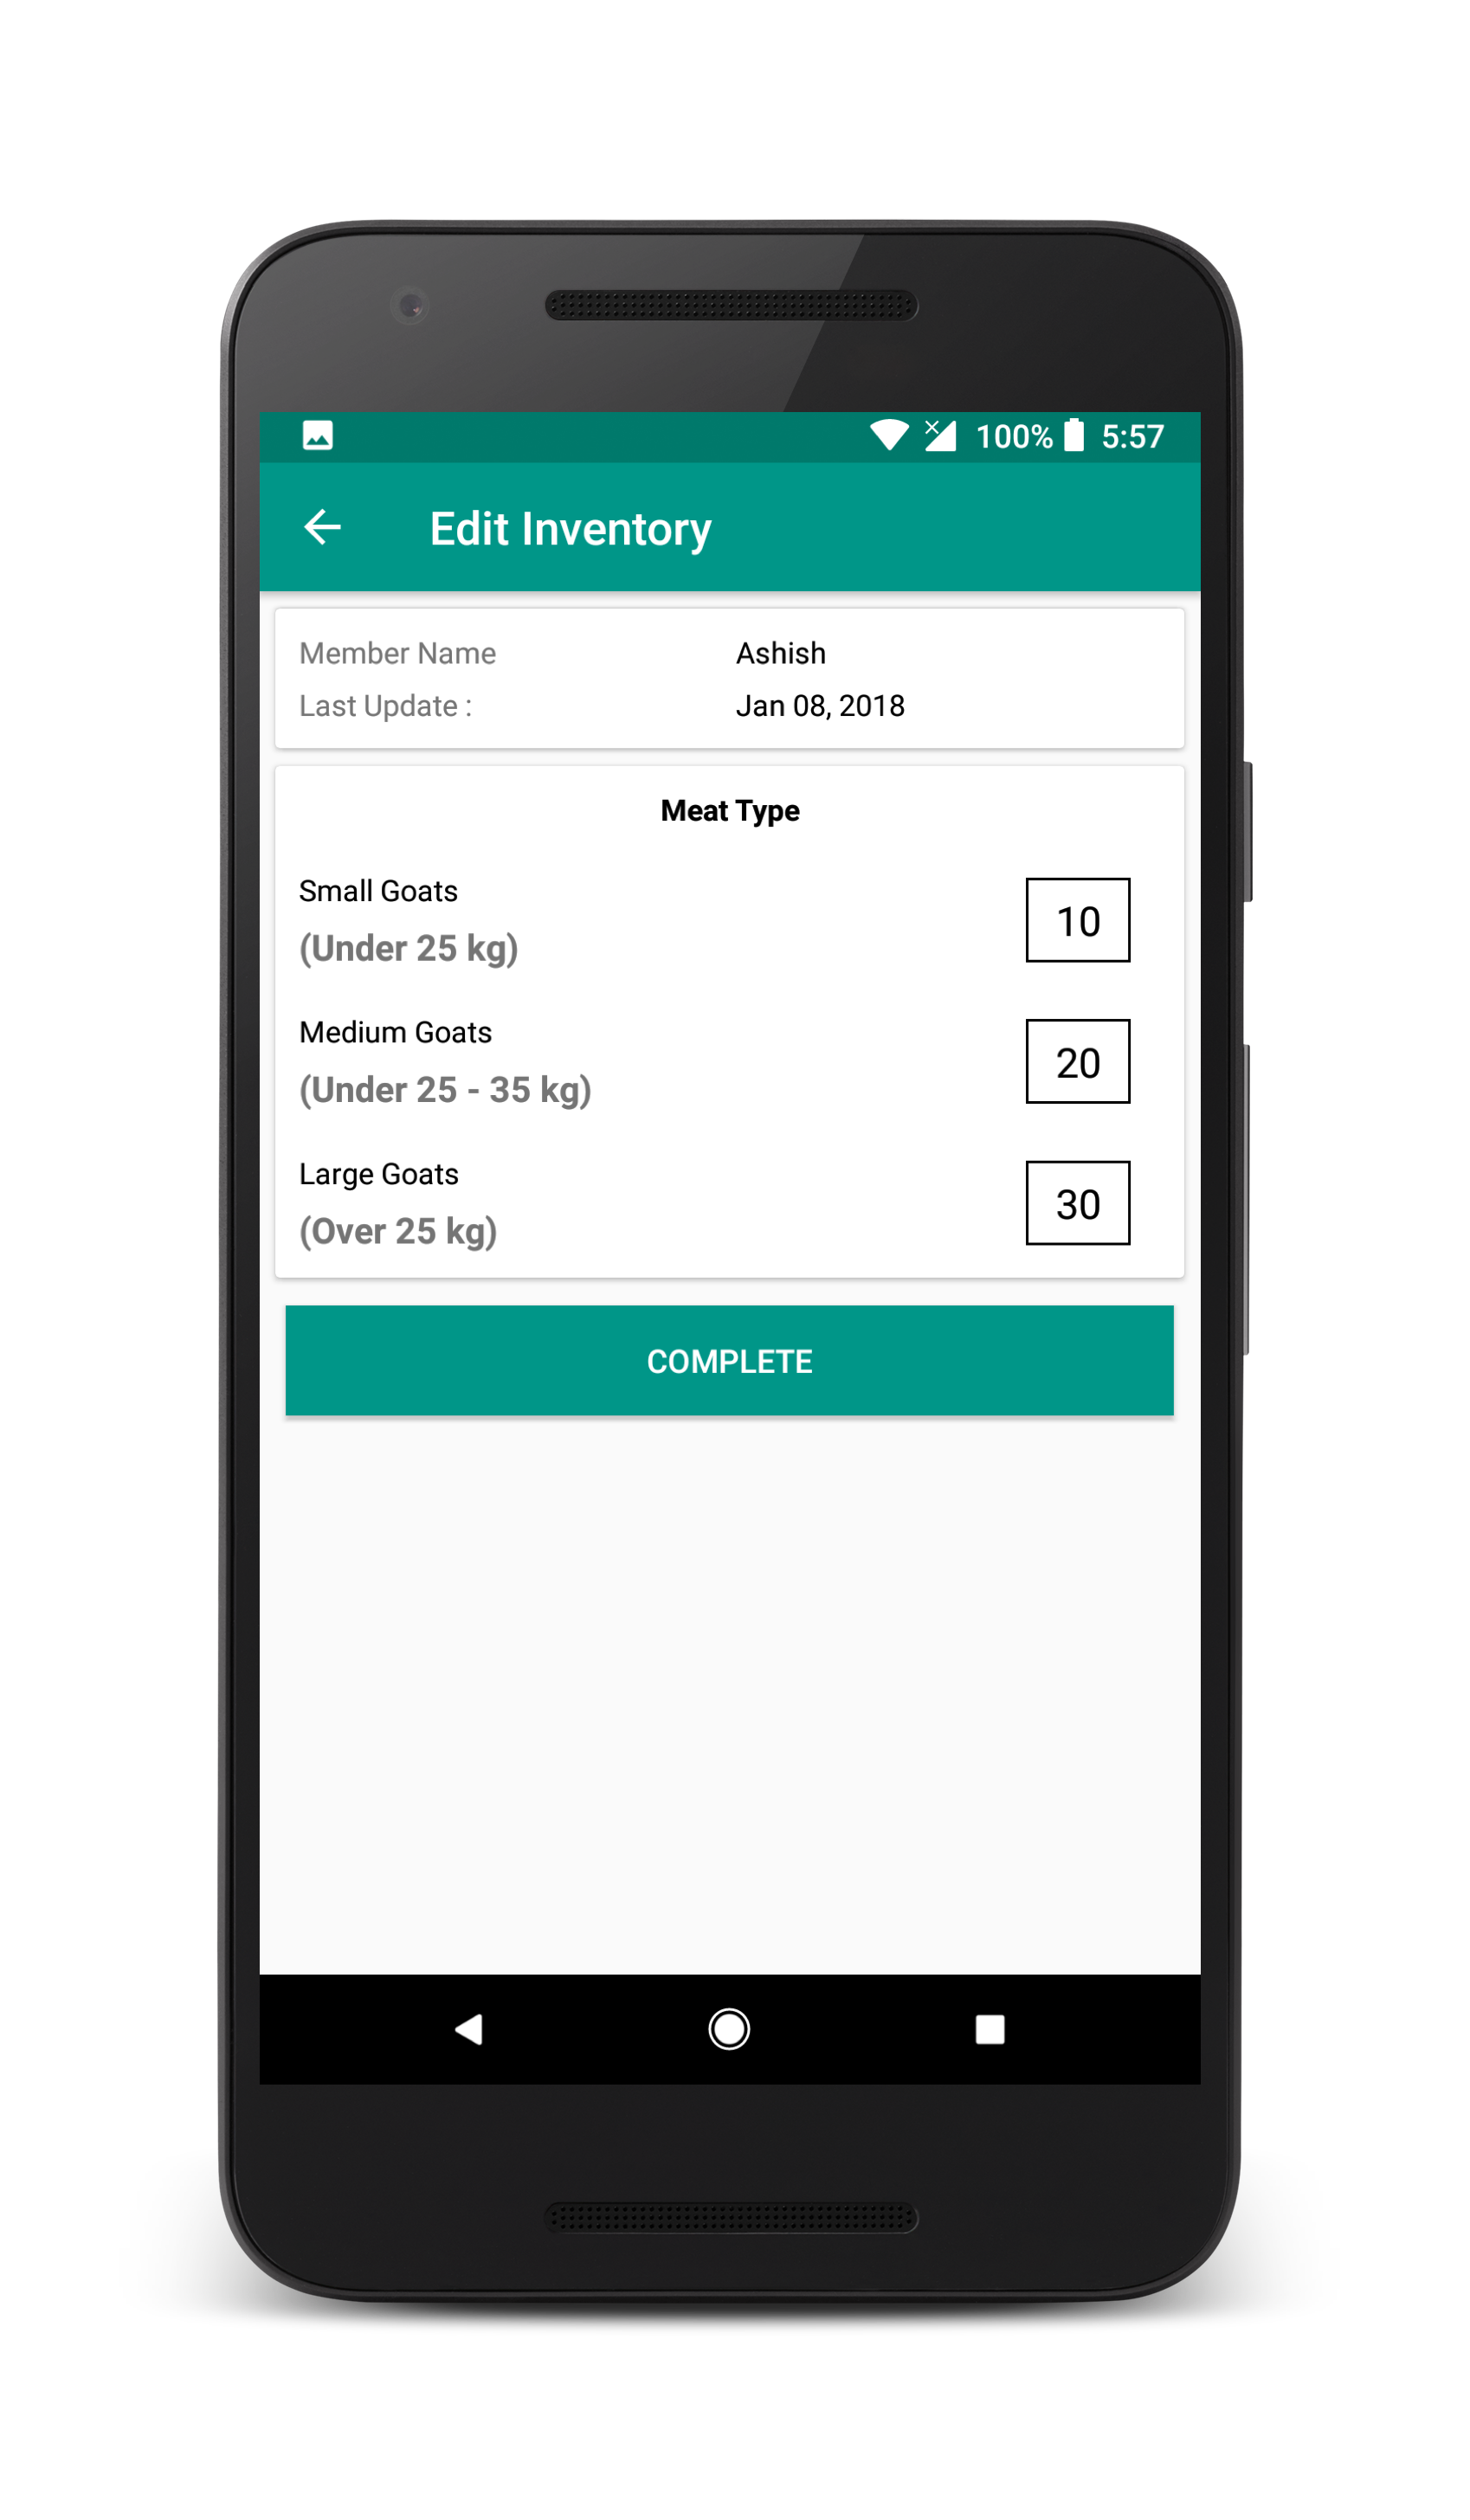
\includegraphics[width=5.7cm]{vcc2.png}
  \end{minipage}
  \hspace{1cm}
  \begin{minipage}{.2\textwidth}
    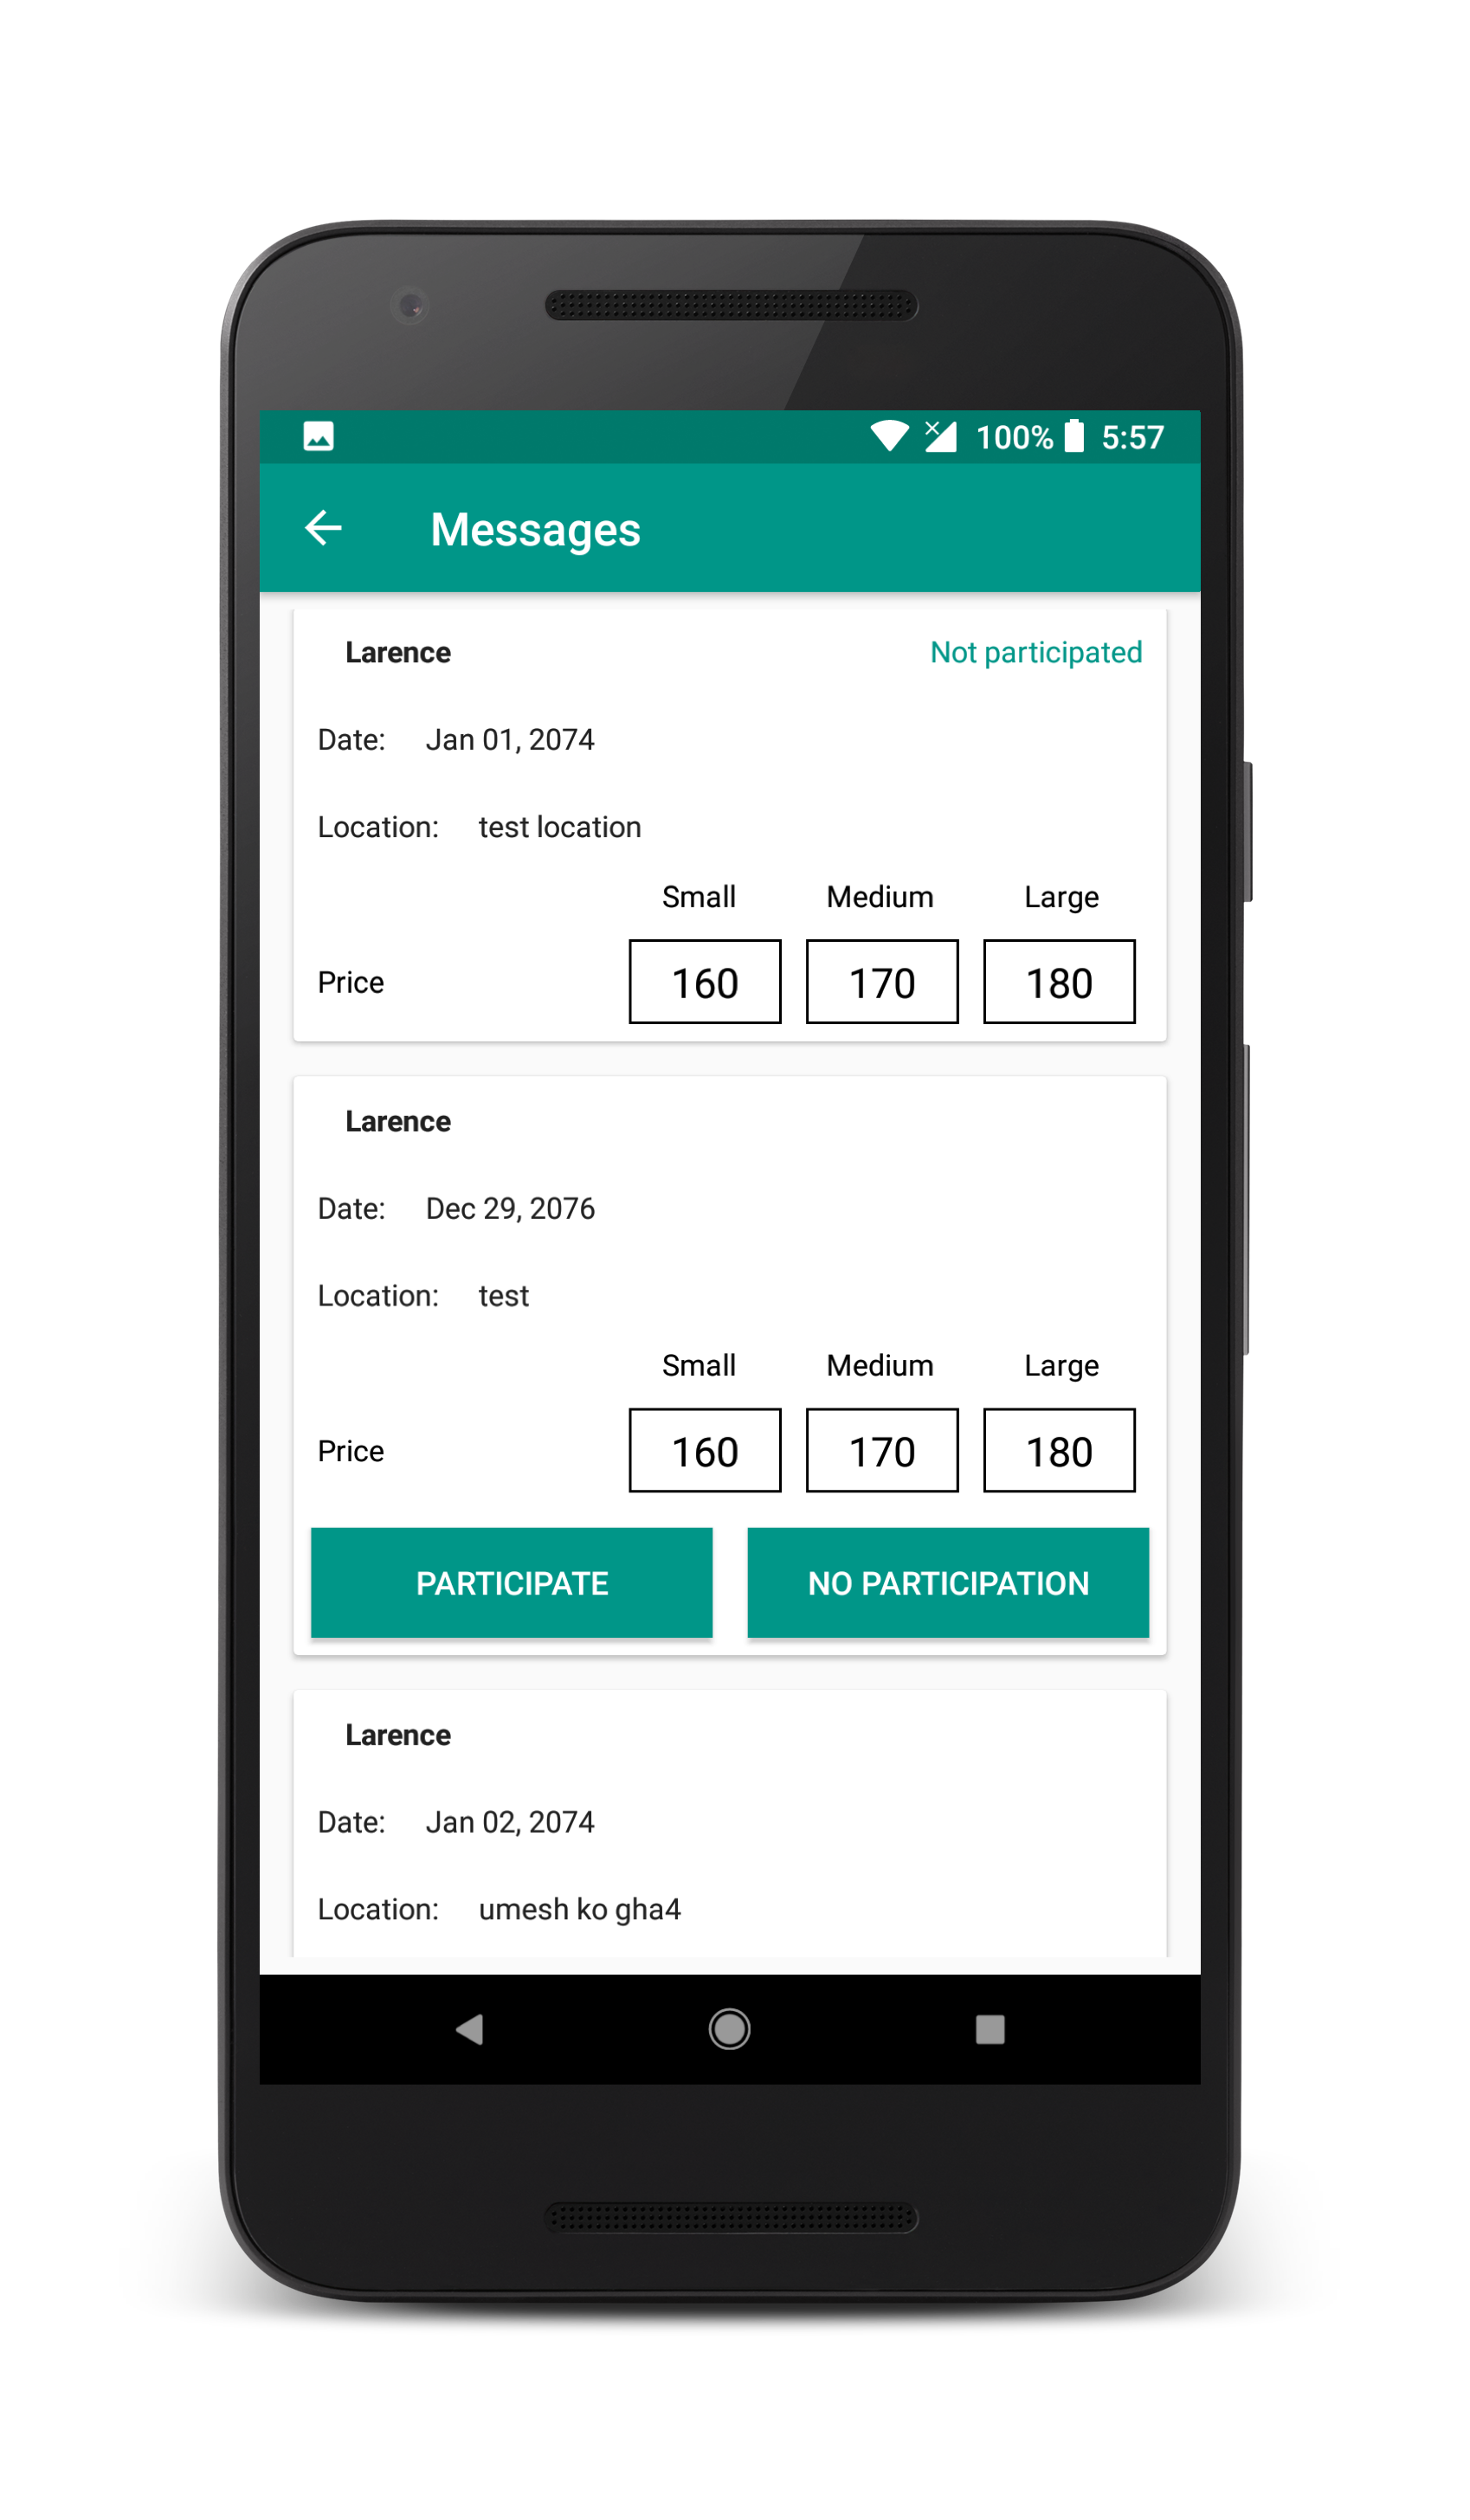
\includegraphics[width=5.7cm]{vcc3.png}
  \end{minipage}
\end{figure}
\end{frame}

\begin{frame}{Essay 3: The Impact of a Smartphone Marketing Application on Smallholder Livestock Producers in Nepal}

\begin{wideitemize}
    \item Estimation strategy for ITT

\begin{equation} \label{eq:ITT1}
y_{ijt} = \rho y_{ijt-1} + \beta_{0} + \beta_{1} T_{j} + \gamma \textbf{S}_{ij} + \varepsilon_{ijt}
\end{equation}
\begin{equation} \label{eq:ITT2}
y_{j} = \rho y_{jt-1} + \beta_{0} + \beta_{1} T_{j} + \gamma \textbf{S}_{j} + \varepsilon_{jt}
\end{equation}

    \vspace{.25cm}
    \begin{itemize}
        \item $y_{ij}$: outcome of interest for household \textit{i} from cooperative \textit{j}. \item $\textbf{S}_{ij}$: indicator variables for the strata created via randomization. \item $T_{j}$: binary treatment indicator
        \item $\beta_{1}$: average intent-to-treat (ITT) effect
            \begin{itemize}
                \item average impact of being given access to the VCC app as well as training on how to use it
            \end{itemize}
    \end{itemize}
\end{wideitemize}
\end{frame}

\begin{frame}{Essay 3: The Impact of a Smartphone Marketing Application on Smallholder Livestock Producers in Nepal}

\begin{wideitemize}
    \item Estimation strategy for heterogeneous treatment effects

\begin{equation} \label{eq:HTE1}
y_{ijt} = \rho y_{ijt-1} + \beta_{0} + \beta_{1} T_{j} + \beta_{2} (T_{j} \times z_{ijt-1}) + \beta_3 z_{ijt-1} + \gamma \textbf{S}_{ij} + \varepsilon_{ijt}
\end{equation}
\begin{equation} \label{eq:HTE2}
y_{j} = \rho y_{jt-1} + \beta_{0} + \beta_{1} T_{j} + \beta_{2} (T_{j} \times z_{jt-1}) + \beta_3 z_{jt-1} + \gamma \textbf{S}_{j} + \varepsilon_{jt}
\end{equation}

    \vspace{.25cm}
    \begin{itemize}
        \item $z_{(i)jt-1}$: household and cooperative characteristics that are hypothesized to have heterogeneous impacts. \vspace{.25cm}
            \begin{enumerate}
                \item Mobile network seriously limits cooperative communication (0/1)
                \item Household sold goats at baseline but not through the cooperative (0/1)
                \item Household sold goats through the cooperative at baseline (0/1)
                \item Round-trip travel time between the household and the cooperative meeting place (minutes - Inverse hyperbolic sine transformation)
            \end{enumerate}
    \end{itemize}
\end{wideitemize}

\end{frame}



% -------------------------------------------------
\begin{frame}
\Huge{\centerline{Questions?}}
\end{frame}

\end{document}

